\section{Locus Triple Winding}

Consider one turn of vertex $P_1(t)$ of billiard 3-periodics around the billiard. Given 3-periodic triple periodicity, over said motion a triangle center will sweep its locus thrice (excluding $X_9$ which doesn't move). To see this, consider what is shown in \cref{fig:05-inc-wind3} where the locus of a convex combination $Y(t)$ of incenter $X_1$ and an intouch point $I(t)$ are shown, namely:

\[ Y(t) = (1-\rho) X_1(t) +  \rho I(t)  \]
where $\rho$ is a real number.

At $\rho=1$ (top-left), $Y(t)$ is the recognizable two-lobe locus of the intouchpoints, shown before in \cref{fig:01-intouch-x59}(left). Since this is the vertex of a derived triangle, each time $P_1(t)$ goes around the outer ellipse, $Y(t)$ winds once around its locus. As  $\rho{\rightarrow}0$, the lobes will (i) approach each other, (ii) become tangent at some threshold (see \cref{ex:05-wind}, (iii) intersect, and at the limit, i.e., when $\rho=0$, the lobes collapse into a single elliptic loop, which by continuity will be wound thrice.

\begin{figure}
    \centering
    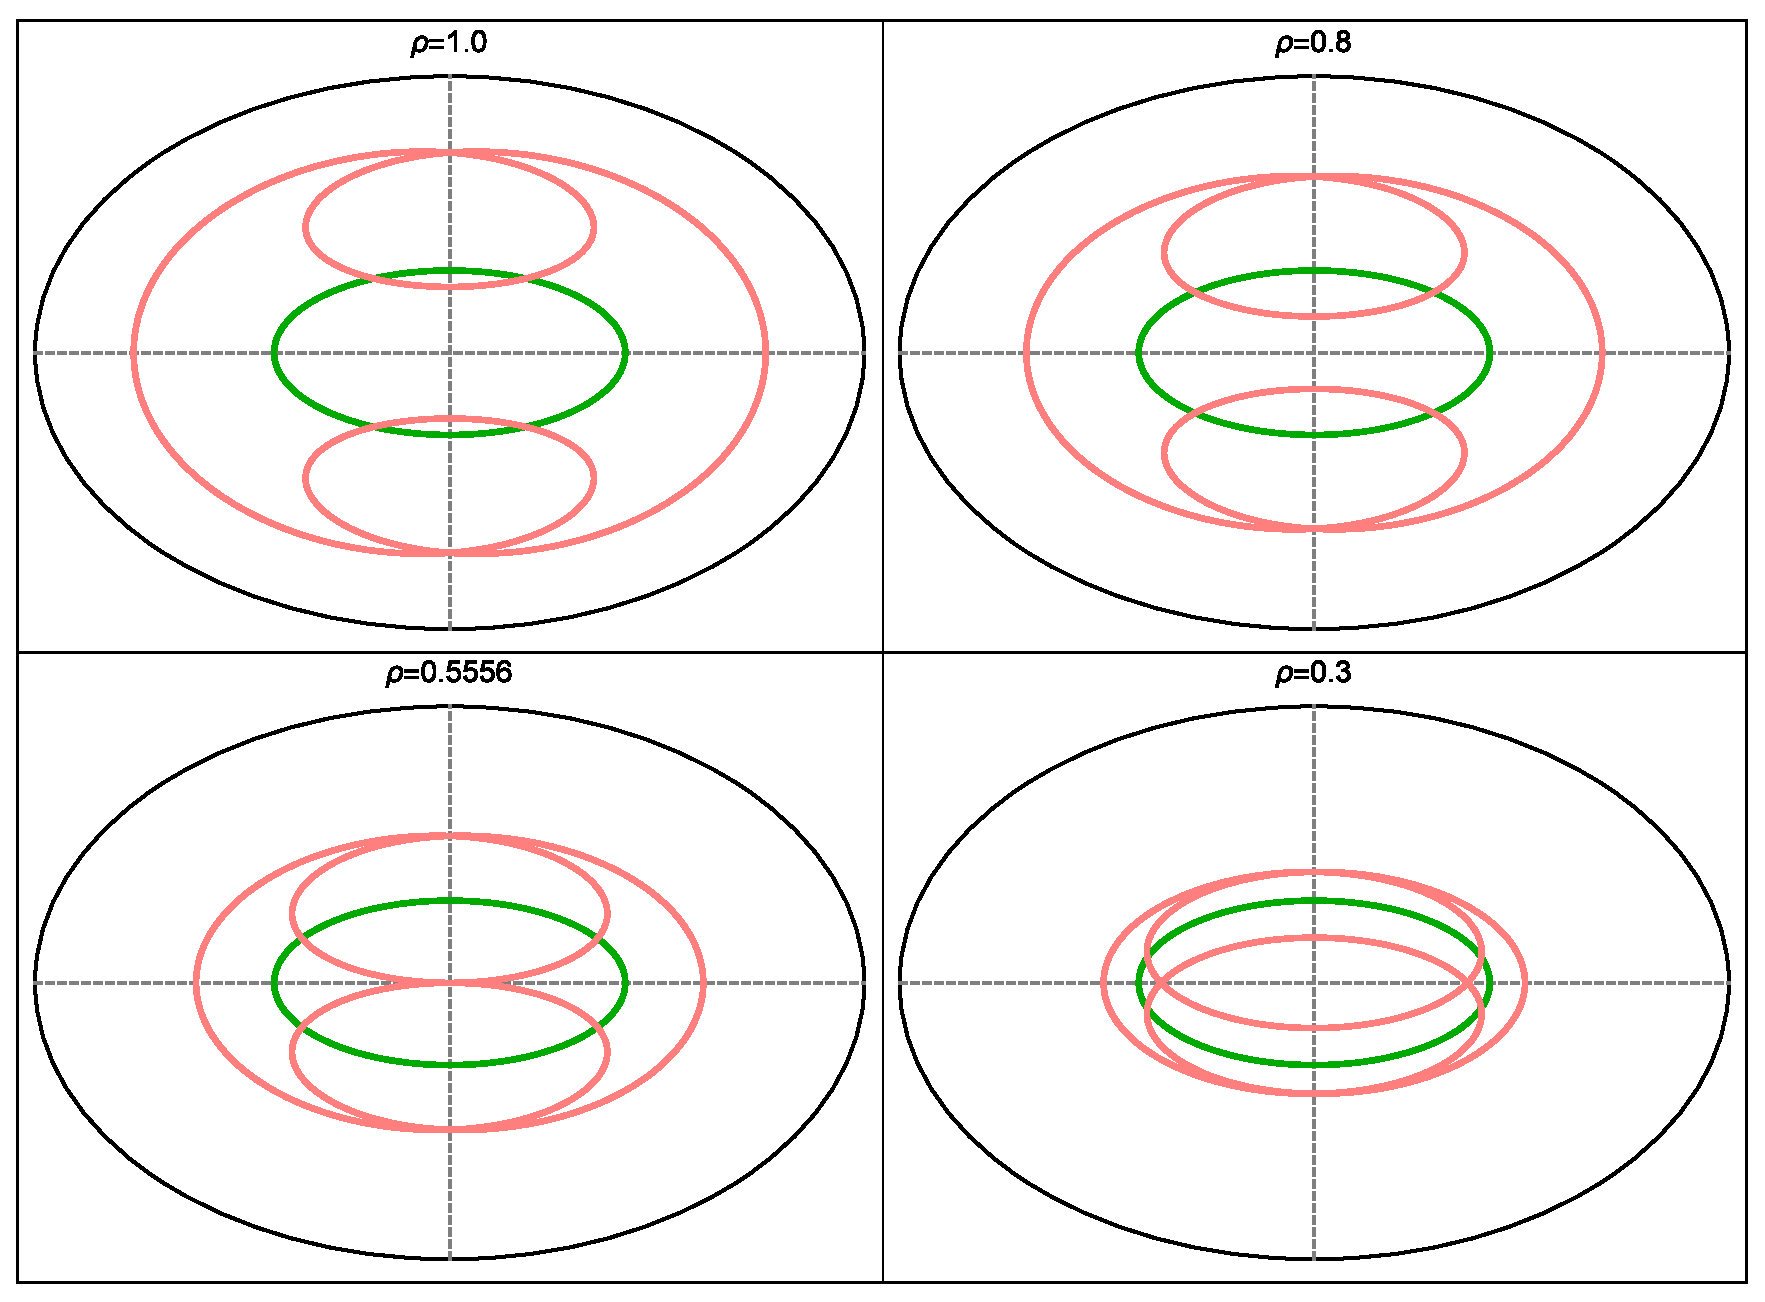
\includegraphics[width=\textwidth]{pics_05_110_conv_inc_pedal}
    \caption{The locus (pink) of a convex combination of an intouchpoint and the incenter for different values of $\rho$. When $\rho=0$ (top left), one obtains the original locus of an intouchpoints. When $\rho=1$ (bottom right), one obtains the elliptic locus of the incenter (green). \href{https://youtu.be/3Gr3Nh5-jHs}{Video 1}, \href{https://youtu.be/HZFjkWD_CnE}{Video 2}}
    \label{fig:05-inc-wind3}
\end{figure}
